%%%%%%%%%%%%%%%%%%%%%%%%%%
%                          %
% ----- INTRODUCTION ----- %
%                          %
%%%%%%%%%%%%%%%%%%%%%%%%%%

\section{Processus de test}

	Une fois toutes les parties du projet réalisées, à savoir l'extension navigateur, le serveur et l'interface, nous avons cherché des utilisateurs volontaires pour installer l'extension et l'utiliser pendant une période de 4 semaines. Bien qu'initialement prévue pour un grand panel d'utilisateurs, les restrictions temporelles ont limité la quantité d'utilisateurs que nous avons pu atteindre.

	Un total de 10 utilisateurs volontaires ont installé l'extension. Parmi eux, 8 ont été identifiés comme ayant une activité de navigation  sur Chrome assez grande pour contribuer à l'étude. (Ceux étant jugés inactifs totalisent moins de 10 minutes d'activité).

	\subsection{Inputs}

		En plus de récolter les données des utilisateurs et de les afficher, il leur a également été demandé de remplir quelques informations sur eux-même afin de pouvoir valider certains points de notre étude. Deux formulaires ont été mis en place à cette fin.

		\subsubsection{Centres d'intérêts}

			La figure~\ref{settings_image} montre un premier formulaire à remplir par l'utilisateur. Accessible via le lien vers la page "Settings", on lui demande ici de trouver et renseigner quelques uns de ces centres d'intérêt parmi une centaine.

			Un maximum de 10 centres d'intérêts peuvent être définis. Le but de laisser à l'utilisateur entrer des centres d'intérêts est de pouvoir nous rendre compte si les topics que nous lui proposons sont proches de ces centres d'intérêt.

		\subsubsection{Association topic et intérêt}

			Une fois que l'utilisateur a défini des centres d'intérêt, il peut donner des informations sur les topics que nous lui suggérons sur la page Topics List (voir section \ref{topicslist}). La figure~\ref{choice} montre la fenêtre déroulante de sélection d'un centre d'intérêt pour un topic donné.

			Il est demandé aux utilisateurs d'ajouter une association entre un topic et un intérêt lorsque cela semble lui faire sens. Ainsi, nous pouvons savoir quels topics de l'utilisateur nous avons réussi à identifier. En effet, lorsqu'un utilisateur associe un centre d'intérêt à un topic, celà signifie non seulement que le topic trouvé a du sens en soi, mais en plus qu'il est intéressant pour l'utilisateur.

			Sur l'échantillon de 8 personnes actives, 6 personnes ont ajouté des associations aux 20 topics proposés sur leur page. 

\section{Evaluation}

	Après une récolte des données sur environ 4 semaines, nous pouvons nous intéresser aux résultats que nous avons récoltés.

	\subsection{Modèles}

		Une première étape est de se pencher sur les modèles que nous avons généré sur la base des données elle-mêmes. Nous utilisons principalement deux algorithmes qui se basent sur le contenu des pages pour en déterminer leur thème : TF-IDF, et LDA.

		Ces modèles se basent sur le contenu des pages visitées des utilisateurs. Etant donné que nous ne récupérons pas directement le contenu de la page visitée par un utilisateur mais uniquement une partie de son URL, nous ne pouvons pas garantir que le contenu que nous récupérons d'une page soit effectivement le contenu que l'utilisateur voit sur son écran. En effet, beaucoup de pages web aujourd'hui sont liées à une application qui demande une authentification de l'utilisateur pour être affichée.

		Par exemple, une grande partie des pages d'un réseau social peuvent nécessiter la connexion de l'utilisateur pour être affichée.

		De plus, il n'existe pas de méthode autre que empiriques pour juger de la qualité des résultats de ce type d'algorithmes. Nous nous attendons donc à des résultats imparfaits, mais allons tenter de juger au mieux leur efficacité malgré ceci.

		\subsubsection{TF-IDF}

			\paragraph{Résultats}

				Le fonctionnement de TF-IDF est décrit à la section \ref{analyse-tfidf}. Juger les résultats du calcul de TF-IDF sur des documents est une tâche non triviale. Cela revient principalement à vérifier manuellement que les mots ayant le poids le plus élevé pour certaines pages soit significatif de leur sujet.

				Intéressons-nous donc aux mots ayant le plus de poids trouvés pour les 20 pages les plus regardées, par exemple. Le tableau\ref{table-tfidf} illustre les 20 pages les plus regardées avec leurs mots associés, ainsi que plusieurs étapes amenant à une estimation finale de l'adéquation des mots trouvés avec le contenu de la page. Voici comment se lit le tableau :
				\begin{description}
					\item[URL] URL de la page concernée. Certaines URLs trop longues ont été raccourcies ici
					\item[Mot 1, 2, 3] 3 meilleurs mots dans l'orrdre décroissant décrivant la page selon TF-IDF.
					\item[Pub(lique)] Est-ce que la page nécessite une connexion afin d'accéder à son contenu principal.
					\item[Con(tenu)] Est-ce que le principal contenu de la page est textuel ?
					\item[Mot] Est-ce que chacun des mots trouvés sur la page fait sens dans une langue connue ?
					\item[Adé(quat)] Est-ce que l'ensemble des mots trouvés forme un potentiel résumé adéquat du contenu de la page ?
				\end{description}

				Les 4 premières colonnes (URL et 3 mots) proviennent de la base de données, tandis que les 4 dernières colonnes sont le résultat d'une évaluation manuelle des critères décrits. Un "OUI" dans une colonne indique que la page a passé le critère défini, contrairement à un "NON". Un "NON" dans une colonne entraîne automatiquement un "NON" dans les colonnes situées les plus à droite.

\begin{sidewaysfigure}
\centering
\caption{20 URLs les plus regardées et leurs meilleurs mots selon TF-IDF}
\label{table-tfidf}
\begin{tabular}{llllllll}
\textbf{URL}                                          & \textbf{Mot 1}  & \textbf{Mot 2}           & \textbf{Mot 3} & \textbf{Pub}           & \textbf{Con}            & \textbf{Mot}               & \textbf{Adé}            \\ \hline
\scriptsize \url{http://wdf.sdipi.ch/}                              & footprints      & digital                  & web            & \cellcolor[HTML]{9AFF99}OUI & \cellcolor[HTML]{9AFF99}OUI & \cellcolor[HTML]{9AFF99}OUI & \cellcolor[HTML]{9AFF99}OUI \\
\scriptsize \url{https://www.draw.io/}                                  & gmdl            & eng                      & proc           & \cellcolor[HTML]{9AFF99}OUI & \cellcolor[HTML]{FFCCC9}NON & \cellcolor[HTML]{FFCCC9}NON & \cellcolor[HTML]{FFCCC9}NON \\
\scriptsize \url{https://www.reddit.com/r/videos/}                      & submit          & load                     & report         & \cellcolor[HTML]{9AFF99}OUI & \cellcolor[HTML]{9AFF99}OUI & \cellcolor[HTML]{9AFF99}OUI & \cellcolor[HTML]{FFCCC9}NON \\
\scriptsize \url{https://www.google.co.uk/search}                       & eingabetaste    & suche                    & drücke         & \cellcolor[HTML]{9AFF99}OUI & \cellcolor[HTML]{FFCCC9}NON & \cellcolor[HTML]{FFCCC9}NON & \cellcolor[HTML]{FFCCC9}NON \\
\scriptsize \url{https://www.google.ch/search}                          & eingabetaste    & suche                    & drücke         & \cellcolor[HTML]{9AFF99}OUI & \cellcolor[HTML]{FFCCC9}NON & \cellcolor[HTML]{FFCCC9}NON & \cellcolor[HTML]{FFCCC9}NON \\
\scriptsize \url{http://game110.idlekiller.com/}                        & explorer        & chrome                   & browser        & \cellcolor[HTML]{9AFF99}OUI & \cellcolor[HTML]{9AFF99}OUI & \cellcolor[HTML]{9AFF99}OUI & \cellcolor[HTML]{9AFF99}OUI \\
\scriptsize \url{http://df.sdipi.ch/phpmyadmin/sql.php}                 & phpmyadmin      & past                     & welcome        & \cellcolor[HTML]{FFCCC9}NON & \cellcolor[HTML]{FFCCC9}NON & \cellcolor[HTML]{FFCCC9}NON & \cellcolor[HTML]{FFCCC9}NON \\
\scriptsize \url{https://web.whatsapp.com/}                             & whatsapp        & macos                    & mozilla        & \cellcolor[HTML]{FFCCC9}NON & \cellcolor[HTML]{FFCCC9}NON & \cellcolor[HTML]{FFCCC9}NON & \cellcolor[HTML]{FFCCC9}NON \\
\scriptsize \url{http://hexaclicker.github.io/}                         & hexa            & dp                       & level          & \cellcolor[HTML]{9AFF99}OUI & \cellcolor[HTML]{9AFF99}OUI & \cellcolor[HTML]{9AFF99}OUI & \cellcolor[HTML]{9AFF99}OUI \\
\scriptsize \url{http://blankmediagames.com/TownOfSalem/}              & salem           & adobe                    & town           & \cellcolor[HTML]{9AFF99}OUI & \cellcolor[HTML]{FFCCC9}NON & \cellcolor[HTML]{FFCCC9}NON & \cellcolor[HTML]{FFCCC9}NON \\
\scriptsize \url{http://www.jeuxvideo.com/}                             & jeu             & annonce                  & bande          & \cellcolor[HTML]{9AFF99}OUI & \cellcolor[HTML]{9AFF99}OUI & \cellcolor[HTML]{9AFF99}OUI & \cellcolor[HTML]{9AFF99}OUI \\
\scriptsize \url{https://discordapp.com/channels/217...408/217...408}   & own             & respective               & owner          & \cellcolor[HTML]{FFCCC9}NON & \cellcolor[HTML]{FFCCC9}NON & \cellcolor[HTML]{FFCCC9}NON & \cellcolor[HTML]{FFCCC9}NON \\
\scriptsize \url{https://www.reddit.com/r/leagueoflegends/}             & leagueoflegends & submit                   & self           & \cellcolor[HTML]{9AFF99}OUI & \cellcolor[HTML]{9AFF99}OUI & \cellcolor[HTML]{9AFF99}OUI & \cellcolor[HTML]{9AFF99}OUI \\
\scriptsize \url{https://www.reddit.com/}                               & bot             & agent                    & pardner        & \cellcolor[HTML]{9AFF99}OUI & \cellcolor[HTML]{9AFF99}OUI & \cellcolor[HTML]{9AFF99}OUI & \cellcolor[HTML]{FFCCC9}NON \\
\scriptsize \url{https://www.google.fr/search}                          & eingabetaste    & suche                    & drücke         & \cellcolor[HTML]{9AFF99}OUI & \cellcolor[HTML]{FFCCC9}NON & \cellcolor[HTML]{FFCCC9}NON & \cellcolor[HTML]{FFCCC9}NON \\
\scriptsize \url{https://s3-fr.gladiatus.gameforge.com/game/index.php}  & de              & gameforge                & vous           & \cellcolor[HTML]{FFCCC9}NON & \cellcolor[HTML]{FFCCC9}NON & \cellcolor[HTML]{FFCCC9}NON & \cellcolor[HTML]{FFCCC9}NON \\
\scriptsize \url{https://docs.google.com/presentation/d/1IB...l5w/edit} & row5w           & gecb...el5w & slide          & \cellcolor[HTML]{FFCCC9}NON & \cellcolor[HTML]{FFCCC9}NON & \cellcolor[HTML]{FFCCC9}NON & \cellcolor[HTML]{FFCCC9}NON \\
\scriptsize \url{https://twitter.com/}                                  & tweet           & foto                     & hast           & \cellcolor[HTML]{9AFF99}OUI & \cellcolor[HTML]{FFCCC9}NON & \cellcolor[HTML]{FFCCC9}NON & \cellcolor[HTML]{FFCCC9}NON \\
\scriptsize \url{http://df.sdipi.ch/phpmyadmin/db\_structure.php}       & phpmyadmin      & past                     & welcome        & \cellcolor[HTML]{FFCCC9}NON & \cellcolor[HTML]{FFCCC9}NON & \cellcolor[HTML]{FFCCC9}NON & \cellcolor[HTML]{FFCCC9}NON \\ \hline
\end{tabular}
\end{sidewaysfigure}

			\paragraph{Réflexion}

				Le fonctionnement de TF-IDF est décrit à la section \ref{analyse-tfidf}. Le tableau~\ref{resultats-tfidf} montre un résumé des résultats que l'on peut récupérer précédent tableau. On remarque que sur les 20 URLs entrées, seules 7 valent vraiment la peine d'être parcourues par notre algorithme, par élimination à causes des deux premières raisons énoncées. Cependant, sur les 7 URLs contenant du texte intéressant, TF-IDF a été capable d'en résumer adéquatement 5 d'entre-elles.

				Ce résultat est loin d'être parfait, mais il montre tout de même qu'il est possible d'automatiser la recherche de mots importants sur des pages lorsque les conditions sont favorables à notre approche.

\FloatBarrier

				\begin{table}[h]
\centering
\caption{Résumé des résultats de TF-IDF}
\label{resultats-tfidf}
\begin{tabular}{lr}
\textbf{URLs initiales}            & 20 \\
\textbf{Pages publiques}           & 14 \\
\textbf{Contenu textuel principal} & 7  \\
\textbf{Mots sensés}               & 7  \\
\textbf{Mots adéquats}             & 5 
\end{tabular}
\end{table}

		\subsubsection{LDA}

			\paragraph{Résultats}

				Dans la première semaine de récolte des résultats, une recherche empirique sur les paramètres à fournir au modèle a été effectuée. Le paramètre du nombre de topics a été fixé à 100; cela semblait un bon compromis, car 50 générait un nombre de trop restreint pour définir de manière assez précise quels étaient les thèmes d'un utisilateur, et 200 générait beaucoup de topics qui n'avaient pas de sens en eux-mêmes.

				Le tableau\ref{table-lda} montre l'ensemble des 100 topics générés, ainsi que plusieurs étapes amenant à une estimation finale de la pertinence tu thème trouvé. Voici comment se lit le tableau :
				\begin{description}
					\item[Mots] 5 meilleurs mots pour décrire le topic
					\item[Mot] Est-ce que chaque mot, pris séparément, a un sens ?
					\item[Thè(me)] Est-ce les mots ont un thème en commun discernable ?
					\item[Thème commun] Quel est le thème en commun des mots ?
					\item[S(e)ns] Est-ce que le thème trouvé peut avoir un sens en tant que centre d'intérêt ?
				\end{description}

				Les mots de la première proviennent de la base de données, tandis que les 4 dernières colonnes sont le résultat d'une évaluation manuelle des critères décrits. Un "OUI" dans une colonne indique que la page a passé le critère défini, contrairement à un "NON". Un "NON" dans une colonne entraîne automatiquement un "NON" dans les colonnes situées les plus à droite.

\begin{longtable}{lllll}
\caption{Topics LDA}\\
\label{table-lda}\\
\textbf{Mots}                                      & \textbf{Mot}                                       & \textbf{Thè}                & \textbf{Thème commun}            & \textbf{Sns}               \\ \hline \endfirsthead
\textbf{Mots}                                      & \textbf{Mot}                                       & \textbf{Thè}                & \textbf{Thème commun}            & \textbf{Sns}               \\ \hline \endhead 
\scriptsize play, n64, subreddit, game, vox                    & \cellcolor[HTML]{9AFF99}OUI & \cellcolor[HTML]{9AFF99}OUI & Jeu vidéo                 & \cellcolor[HTML]{9AFF99}OUI \\
\scriptsize add, ad, free, div, class                          & \cellcolor[HTML]{9AFF99}OUI & \cellcolor[HTML]{FFCCC9}NON & -                         & \cellcolor[HTML]{FFCCC9}NON \\
\scriptsize game, studio, software, entertainment, ... & \cellcolor[HTML]{9AFF99}OUI & \cellcolor[HTML]{9AFF99}OUI & Dévelop. jeu vidéo            & \cellcolor[HTML]{9AFF99}OUI \\
\scriptsize dog, sign, dogbuddy, amp, style                    & \cellcolor[HTML]{9AFF99}OUI & \cellcolor[HTML]{FFCCC9}NON & -                         & \cellcolor[HTML]{FFCCC9}NON \\
\scriptsize vue, component, data, will, render                 & \cellcolor[HTML]{9AFF99}OUI & \cellcolor[HTML]{9AFF99}OUI & Vue.js framework          & \cellcolor[HTML]{9AFF99}OUI \\
\scriptsize example, vector, product, displaystyle, cross      & \cellcolor[HTML]{9AFF99}OUI & \cellcolor[HTML]{9AFF99}OUI & Librairie de graphes      & \cellcolor[HTML]{9AFF99}OUI \\
\scriptsize please, browser, javascript, intel, vi             & \cellcolor[HTML]{9AFF99}OUI & \cellcolor[HTML]{FFCCC9}NON & -                         & \cellcolor[HTML]{FFCCC9}NON \\
\scriptsize self, topic, word, model, corpus                   & \cellcolor[HTML]{9AFF99}OUI & \cellcolor[HTML]{9AFF99}OUI & Topic modelling           & \cellcolor[HTML]{9AFF99}OUI \\
\scriptsize antwort, google, bleiben, div, thema               & \cellcolor[HTML]{9AFF99}OUI & \cellcolor[HTML]{FFCCC9}NON & -                         & \cellcolor[HTML]{FFCCC9}NON \\
\scriptsize chf, prix, km, ch, gris                            & \cellcolor[HTML]{9AFF99}OUI & \cellcolor[HTML]{FFCCC9}NON & -                         & \cellcolor[HTML]{FFCCC9}NON \\
\scriptsize chrome, api, web, devtools, headless               & \cellcolor[HTML]{9AFF99}OUI & \cellcolor[HTML]{9AFF99}OUI & Chrome API                & \cellcolor[HTML]{9AFF99}OUI \\
\scriptsize github, sign, data, issue, tab                     & \cellcolor[HTML]{9AFF99}OUI & \cellcolor[HTML]{9AFF99}OUI & Github                    & \cellcolor[HTML]{9AFF99}OUI \\
\scriptsize also, system, love, note, may                      & \cellcolor[HTML]{9AFF99}OUI & \cellcolor[HTML]{FFCCC9}NON & -                         & \cellcolor[HTML]{FFCCC9}NON \\
\scriptsize view, u, duration, minute, add                     & \cellcolor[HTML]{9AFF99}OUI & \cellcolor[HTML]{FFCCC9}NON & -                         & \cellcolor[HTML]{FFCCC9}NON \\
\scriptsize jan, oct, dec, nov, feb                            & \cellcolor[HTML]{9AFF99}OUI & \cellcolor[HTML]{9AFF99}OUI & Mois de l'année           & \cellcolor[HTML]{FFCCC9}NON \\
\scriptsize v0, td, selectize, class, nowrap                   & \cellcolor[HTML]{9AFF99}OUI & \cellcolor[HTML]{9AFF99}OUI & Librairie JS              & \cellcolor[HTML]{9AFF99}OUI \\
\scriptsize laptop, lenovo, driver, thinkpad, nvidia           & \cellcolor[HTML]{9AFF99}OUI & \cellcolor[HTML]{9AFF99}OUI & Produits Lenovo           & \cellcolor[HTML]{9AFF99}OUI \\
\scriptsize vue, composant, composants, propriétés, ...    & \cellcolor[HTML]{9AFF99}OUI & \cellcolor[HTML]{9AFF99}OUI & Vue.js framework          & \cellcolor[HTML]{9AFF99}OUI \\
\scriptsize point, reply, child, give, permalink               & \cellcolor[HTML]{9AFF99}OUI & \cellcolor[HTML]{9AFF99}OUI & Reddit                    & \cellcolor[HTML]{9AFF99}OUI \\
\scriptsize support, english, product, security, steam         & \cellcolor[HTML]{9AFF99}OUI & \cellcolor[HTML]{FFCCC9}NON & -                         & \cellcolor[HTML]{FFCCC9}NON \\
\scriptsize school, child, social, research, study             & \cellcolor[HTML]{9AFF99}OUI & \cellcolor[HTML]{9AFF99}OUI & Ecole                     & \cellcolor[HTML]{9AFF99}OUI \\
\scriptsize facebook, retweets, registrieren, seite, konto     & \cellcolor[HTML]{9AFF99}OUI & \cellcolor[HTML]{9AFF99}OUI & Réseaux sociaux           & \cellcolor[HTML]{9AFF99}OUI \\
\scriptsize kid, baby, girl, child, parent                     & \cellcolor[HTML]{9AFF99}OUI & \cellcolor[HTML]{9AFF99}OUI & Enfants                   & \cellcolor[HTML]{9AFF99}OUI \\
\scriptsize kindle, commentaire, the, produit, amazon          & \cellcolor[HTML]{9AFF99}OUI & \cellcolor[HTML]{9AFF99}OUI & Produits Amazon           & \cellcolor[HTML]{9AFF99}OUI \\
\scriptsize root, size, review, id, common                     & \cellcolor[HTML]{9AFF99}OUI & \cellcolor[HTML]{FFCCC9}NON & -                         & \cellcolor[HTML]{FFCCC9}NON \\
\scriptsize string, type, return, class, json                  & \cellcolor[HTML]{9AFF99}OUI & \cellcolor[HTML]{9AFF99}OUI & Types JSON                & \cellcolor[HTML]{FFCCC9}NON \\
\scriptsize twitter, gefällt, account, antworten, tweets       & \cellcolor[HTML]{9AFF99}OUI & \cellcolor[HTML]{9AFF99}OUI & Twitter                   & \cellcolor[HTML]{9AFF99}OUI \\
\scriptsize plus, bien, autres, voir, jour                     & \cellcolor[HTML]{9AFF99}OUI & \cellcolor[HTML]{FFCCC9}NON & -                         & \cellcolor[HTML]{FFCCC9}NON \\
\scriptsize ago, year, month, day, switch                      & \cellcolor[HTML]{9AFF99}OUI & \cellcolor[HTML]{9AFF99}OUI & Durée                     & \cellcolor[HTML]{FFCCC9}NON \\
\scriptsize leagueoflegends, champion, http, img, png          & \cellcolor[HTML]{9AFF99}OUI & \cellcolor[HTML]{9AFF99}OUI & League of Legends         & \cellcolor[HTML]{9AFF99}OUI \\
\scriptsize webpack, j, loader, file, module                   & \cellcolor[HTML]{9AFF99}OUI & \cellcolor[HTML]{9AFF99}OUI & Webpack                   & \cellcolor[HTML]{9AFF99}OUI \\
\scriptsize replay, del, normal, lunatic, extra                & \cellcolor[HTML]{9AFF99}OUI & \cellcolor[HTML]{9AFF99}OUI & Niveaux de jeu vidéo      & \cellcolor[HTML]{9AFF99}OUI \\
\scriptsize the, ch, hast, to, and                             & \cellcolor[HTML]{FFCCC9}NON & \cellcolor[HTML]{FFCCC9}NON & -                         & \cellcolor[HTML]{FFCCC9}NON \\
\scriptsize amazon, game, badge, book, home                    & \cellcolor[HTML]{9AFF99}OUI & \cellcolor[HTML]{FFCCC9}NON & -                         & \cellcolor[HTML]{FFCCC9}NON \\
\scriptsize window, microsoft, windows, store, phantomjs       & \cellcolor[HTML]{9AFF99}OUI & \cellcolor[HTML]{9AFF99}OUI & Windows                   & \cellcolor[HTML]{9AFF99}OUI \\
\scriptsize property, method, data, server, application        & \cellcolor[HTML]{9AFF99}OUI & \cellcolor[HTML]{9AFF99}OUI & Dev. backend              & \cellcolor[HTML]{9AFF99}OUI \\
\scriptsize yes, flag, prototype, array, strict                & \cellcolor[HTML]{9AFF99}OUI & \cellcolor[HTML]{FFCCC9}NON & -                         & \cellcolor[HTML]{FFCCC9}NON \\
\scriptsize post, publish, revision, code, microspot           & \cellcolor[HTML]{9AFF99}OUI & \cellcolor[HTML]{FFCCC9}NON & -                         & \cellcolor[HTML]{FFCCC9}NON \\
\scriptsize zelda, wild, breath, link, legend                  & \cellcolor[HTML]{9AFF99}OUI & \cellcolor[HTML]{9AFF99}OUI & The Legend of Zelda       & \cellcolor[HTML]{9AFF99}OUI \\
\scriptsize head, coin, room, stone, ll                        & \cellcolor[HTML]{9AFF99}OUI & \cellcolor[HTML]{FFCCC9}NON & -                         & \cellcolor[HTML]{FFCCC9}NON \\
\scriptsize icon, copy, font, arrow, fill                      & \cellcolor[HTML]{9AFF99}OUI & \cellcolor[HTML]{9AFF99}OUI & Graphisme                 & \cellcolor[HTML]{9AFF99}OUI \\
\scriptsize modifier, code, états, unis, article               & \cellcolor[HTML]{9AFF99}OUI & \cellcolor[HTML]{9AFF99}OUI & Article Etats-Unis        & \cellcolor[HTML]{9AFF99}OUI \\
\scriptsize class, div, html, cs, button                       & \cellcolor[HTML]{9AFF99}OUI & \cellcolor[HTML]{9AFF99}OUI & Elements HTML             & \cellcolor[HTML]{9AFF99}OUI \\
\scriptsize child, food, see, year, book                       & \cellcolor[HTML]{9AFF99}OUI & \cellcolor[HTML]{FFCCC9}NON & -                         & \cellcolor[HTML]{FFCCC9}NON \\
\scriptsize cuisinières, min, laver, service, cuisson          & \cellcolor[HTML]{9AFF99}OUI & \cellcolor[HTML]{9AFF99}OUI & Cuisine                   & \cellcolor[HTML]{9AFF99}OUI \\
\scriptsize time, season, episode, adventure, part             & \cellcolor[HTML]{9AFF99}OUI & \cellcolor[HTML]{9AFF99}OUI & Série télévisée           & \cellcolor[HTML]{9AFF99}OUI \\
\scriptsize image, png, data, width, item                      & \cellcolor[HTML]{9AFF99}OUI & \cellcolor[HTML]{9AFF99}OUI & Métadonnées image         & \cellcolor[HTML]{9AFF99}OUI \\
\scriptsize mysql, syntax, table, statement, create            & \cellcolor[HTML]{9AFF99}OUI & \cellcolor[HTML]{9AFF99}OUI & SQL                       & \cellcolor[HTML]{9AFF99}OUI \\
\scriptsize account, sign, email, please, click                & \cellcolor[HTML]{9AFF99}OUI & \cellcolor[HTML]{9AFF99}OUI & Compte mail               & \cellcolor[HTML]{9AFF99}OUI \\
\scriptsize url, request, flask, app, response                 & \cellcolor[HTML]{9AFF99}OUI & \cellcolor[HTML]{9AFF99}OUI & Flask Framework           & \cellcolor[HTML]{9AFF99}OUI \\
\scriptsize chart, plot, data, column, babish                  & \cellcolor[HTML]{9AFF99}OUI & \cellcolor[HTML]{9AFF99}OUI & Graphique                 & \cellcolor[HTML]{9AFF99}OUI \\
\scriptsize video, youtube, watch, vimeo, makeup               & \cellcolor[HTML]{9AFF99}OUI & \cellcolor[HTML]{9AFF99}OUI & Vidéo                     & \cellcolor[HTML]{9AFF99}OUI \\
\scriptsize file, npm, package, run, version                   & \cellcolor[HTML]{9AFF99}OUI & \cellcolor[HTML]{9AFF99}OUI & Packaging application     & \cellcolor[HTML]{9AFF99}OUI \\
\scriptsize date, prototype, support, object, document         & \cellcolor[HTML]{9AFF99}OUI & \cellcolor[HTML]{FFCCC9}NON & -                         & \cellcolor[HTML]{FFCCC9}NON \\
\scriptsize function, var, return, array, option               & \cellcolor[HTML]{9AFF99}OUI & \cellcolor[HTML]{9AFF99}OUI & Keywords (prog)           & \cellcolor[HTML]{9AFF99}OUI \\
\scriptsize light, book, lamp, night, éclairage                & \cellcolor[HTML]{9AFF99}OUI & \cellcolor[HTML]{9AFF99}OUI & Lumière                   & \cellcolor[HTML]{9AFF99}OUI \\
\scriptsize answer, stack, vote, overflow, question            & \cellcolor[HTML]{9AFF99}OUI & \cellcolor[HTML]{9AFF99}OUI & StackOverflow             & \cellcolor[HTML]{9AFF99}OUI \\
\scriptsize like, get, just, one, make                         & \cellcolor[HTML]{9AFF99}OUI & \cellcolor[HTML]{FFCCC9}NON & -                         & \cellcolor[HTML]{FFCCC9}NON \\
\scriptsize flex, div, align, item, content                    & \cellcolor[HTML]{9AFF99}OUI & \cellcolor[HTML]{9AFF99}OUI & CSS                       & \cellcolor[HTML]{9AFF99}OUI \\
\scriptsize typescript, code, test, type, file                 & \cellcolor[HTML]{9AFF99}OUI & \cellcolor[HTML]{9AFF99}OUI & TypeScript                & \cellcolor[HTML]{9AFF99}OUI \\
\scriptsize thread, method, call, will, module                 & \cellcolor[HTML]{9AFF99}OUI & \cellcolor[HTML]{9AFF99}OUI & Concurrence (prog)        & \cellcolor[HTML]{9AFF99}OUI \\
\scriptsize character, draw, art, design, forward              & \cellcolor[HTML]{9AFF99}OUI & \cellcolor[HTML]{9AFF99}OUI & Personnage fiction        & \cellcolor[HTML]{9AFF99}OUI \\
\scriptsize amazon, plus, prime, jeux, nav                     & \cellcolor[HTML]{9AFF99}OUI & \cellcolor[HTML]{9AFF99}OUI & Produits Amazon           & \cellcolor[HTML]{9AFF99}OUI \\
\scriptsize option, value, select, input, label                & \cellcolor[HTML]{9AFF99}OUI & \cellcolor[HTML]{9AFF99}OUI & Formulaire HTML           & \cellcolor[HTML]{9AFF99}OUI \\
\scriptsize table, td, th, silhouette, tr                      & \cellcolor[HTML]{9AFF99}OUI & \cellcolor[HTML]{9AFF99}OUI & Tableau HTML              & \cellcolor[HTML]{9AFF99}OUI \\
\scriptsize hsbc, business, banking, website, http             & \cellcolor[HTML]{9AFF99}OUI & \cellcolor[HTML]{9AFF99}OUI & E-Banking                 & \cellcolor[HTML]{9AFF99}OUI \\
\scriptsize november, history, world, december, retrieve       & \cellcolor[HTML]{9AFF99}OUI & \cellcolor[HTML]{FFCCC9}NON & -                         & \cellcolor[HTML]{FFCCC9}NON \\
\scriptsize anime, girl, manga, meme, irl                      & \cellcolor[HTML]{9AFF99}OUI & \cellcolor[HTML]{9AFF99}OUI & Anime                     & \cellcolor[HTML]{9AFF99}OUI \\
\scriptsize top, middle, support, jungle, stockage             & \cellcolor[HTML]{9AFF99}OUI & \cellcolor[HTML]{9AFF99}OUI & Rôles (League of Legends) & \cellcolor[HTML]{9AFF99}OUI \\
\scriptsize net, number, random, insert, openx                 & \cellcolor[HTML]{9AFF99}OUI & \cellcolor[HTML]{9AFF99}OUI & Nombres                   & \cellcolor[HTML]{FFCCC9}NON \\
\scriptsize advertising, design, ad, forward, marketing        & \cellcolor[HTML]{9AFF99}OUI & \cellcolor[HTML]{9AFF99}OUI & Marketing                 & \cellcolor[HTML]{9AFF99}OUI \\
\scriptsize channel, message, princess, margaret, jump         & \cellcolor[HTML]{9AFF99}OUI & \cellcolor[HTML]{FFCCC9}NON & -                         & \cellcolor[HTML]{FFCCC9}NON \\
\scriptsize accessoires, cm, autres, iphone, jeux              & \cellcolor[HTML]{9AFF99}OUI & \cellcolor[HTML]{FFCCC9}NON & -                         & \cellcolor[HTML]{FFCCC9}NON \\
\scriptsize canada, québec, france, ainsi, guerre              & \cellcolor[HTML]{9AFF99}OUI & \cellcolor[HTML]{9AFF99}OUI & Pays                      & \cellcolor[HTML]{FFCCC9}NON \\
\scriptsize merci, janvier, classe, enfants, répondre          & \cellcolor[HTML]{9AFF99}OUI & \cellcolor[HTML]{FFCCC9}NON & -                         & \cellcolor[HTML]{FFCCC9}NON \\
\scriptsize de, la, le, nutzt, kommentare                      & \cellcolor[HTML]{9AFF99}OUI & \cellcolor[HTML]{FFCCC9}NON & -                         & \cellcolor[HTML]{FFCCC9}NON \\
\scriptsize vaisselle, poche, tuner, longueur, gcn             & \cellcolor[HTML]{9AFF99}OUI & \cellcolor[HTML]{FFCCC9}NON & -                         & \cellcolor[HTML]{FFCCC9}NON \\
\scriptsize page, edit, fire, hero, list                       & \cellcolor[HTML]{9AFF99}OUI & \cellcolor[HTML]{FFCCC9}NON & -                         & \cellcolor[HTML]{FFCCC9}NON \\
\scriptsize stock, temp, come, soon, sell                      & \cellcolor[HTML]{9AFF99}OUI & \cellcolor[HTML]{9AFF99}OUI & Bourse                    & \cellcolor[HTML]{9AFF99}OUI \\
\scriptsize jeu, amp, ps4, pc, jeux                            & \cellcolor[HTML]{9AFF99}OUI & \cellcolor[HTML]{9AFF99}OUI & Jeux vidéo                & \cellcolor[HTML]{9AFF99}OUI \\
\scriptsize pm, january, follow, http, www                     & \cellcolor[HTML]{9AFF99}OUI & \cellcolor[HTML]{FFCCC9}NON & -                         & \cellcolor[HTML]{FFCCC9}NON \\
\scriptsize img, src, alt, http, jpg                           & \cellcolor[HTML]{9AFF99}OUI & \cellcolor[HTML]{9AFF99}OUI & Métadonnées image         & \cellcolor[HTML]{9AFF99}OUI \\
\scriptsize net, post, internet, neutrality, trump             & \cellcolor[HTML]{9AFF99}OUI & \cellcolor[HTML]{9AFF99}OUI & Net neutrality            & \cellcolor[HTML]{9AFF99}OUI \\
\scriptsize comment, reddit, post, save, report                & \cellcolor[HTML]{9AFF99}OUI & \cellcolor[HTML]{9AFF99}OUI & Reddit                    & \cellcolor[HTML]{9AFF99}OUI \\
\scriptsize game, card, switch, update, now                    & \cellcolor[HTML]{9AFF99}OUI & \cellcolor[HTML]{9AFF99}OUI & Jeu vidéo                 & \cellcolor[HTML]{9AFF99}OUI \\
\scriptsize game, league, team, legend, comment                & \cellcolor[HTML]{9AFF99}OUI & \cellcolor[HTML]{9AFF99}OUI & League of Legends         & \cellcolor[HTML]{9AFF99}OUI \\
\scriptsize nintendo, switch, mario, demande, iwata            & \cellcolor[HTML]{9AFF99}OUI & \cellcolor[HTML]{9AFF99}OUI & Nintendo                  & \cellcolor[HTML]{9AFF99}OUI \\
\scriptsize pack, ce, café, news, bbc                          & \cellcolor[HTML]{9AFF99}OUI & \cellcolor[HTML]{FFCCC9}NON & -                         & \cellcolor[HTML]{FFCCC9}NON \\
\scriptsize reimu, interest, manipulation, shrine, touhou      & \cellcolor[HTML]{9AFF99}OUI & \cellcolor[HTML]{9AFF99}OUI & Touhou Project            & \cellcolor[HTML]{9AFF99}OUI \\
\scriptsize moon, blood, tattoo, artwork, madj0hn              & \cellcolor[HTML]{9AFF99}OUI & \cellcolor[HTML]{9AFF99}OUI & Tatouages                 & \cellcolor[HTML]{9AFF99}OUI \\
\scriptsize select, mysql, set, value, sql                     & \cellcolor[HTML]{9AFF99}OUI & \cellcolor[HTML]{9AFF99}OUI & SQL                       & \cellcolor[HTML]{9AFF99}OUI \\
\scriptsize amp, google, web, android, app                     & \cellcolor[HTML]{9AFF99}OUI & \cellcolor[HTML]{9AFF99}OUI & Android                   & \cellcolor[HTML]{9AFF99}OUI \\
\scriptsize amp, log, src, hide, style                         & \cellcolor[HTML]{9AFF99}OUI & \cellcolor[HTML]{FFCCC9}NON & -                         & \cellcolor[HTML]{FFCCC9}NON \\
\scriptsize eps3, robot, mr, season, wiki                      & \cellcolor[HTML]{9AFF99}OUI & \cellcolor[HTML]{9AFF99}OUI & Mr.Robot                  & \cellcolor[HTML]{9AFF99}OUI \\
\scriptsize suisse, protecteur, vapeur, services, sécurité     & \cellcolor[HTML]{9AFF99}OUI & \cellcolor[HTML]{9AFF99}OUI & Sécurité                  & \cellcolor[HTML]{9AFF99}OUI \\
\scriptsize rate, earn, win, th, panda                         & \cellcolor[HTML]{9AFF99}OUI & \cellcolor[HTML]{FFCCC9}NON & -                         & \cellcolor[HTML]{FFCCC9}NON \\
\scriptsize share, facebook, link, pinterest, twitter          & \cellcolor[HTML]{9AFF99}OUI & \cellcolor[HTML]{9AFF99}OUI & Réseaux sociaux           & \cellcolor[HTML]{9AFF99}OUI \\
\scriptsize function, class, name, object, decorator           & \cellcolor[HTML]{9AFF99}OUI & \cellcolor[HTML]{9AFF99}OUI & Fonction (prog)           & \cellcolor[HTML]{FFCCC9}NON \\
\scriptsize unit, attack, build, hero, hp                      & \cellcolor[HTML]{9AFF99}OUI & \cellcolor[HTML]{9AFF99}OUI & Theorycraft               & \cellcolor[HTML]{9AFF99}OUI \\
\scriptsize the, saison, série, big, film                      & \cellcolor[HTML]{9AFF99}OUI & \cellcolor[HTML]{9AFF99}OUI & Télévision                & \cellcolor[HTML]{9AFF99}OUI
\end{longtable}

			\paragraph{Réflexion}

				Le fonctionnement de LDA est décrit à la section \ref{analyse-lda}. Le tableau~\ref{resultats-lda} montre un résumé des résultats que l'on peut récupérer précédent tableau. Sur les 100 topics générés par le modèle, on a pu estimer qu'au final 65 de ceux-ci sont des topics potentiellement désirables, et décrivant un thème commun et sensé.

				\FloatBarrier

\begin{table}[h]
\centering
\caption{Résumé des résultats de LDA}
\label{resultats-lda}
\begin{tabular}{lr}
\textbf{Topics générés}            & 100 \\
\textbf{avec mots sensés}           & 99 \\
\textbf{avec un topic commun}       & 71 \\
\textbf{avec un topic sensé}        & 65 \\
\end{tabular}
\end{table}

				Bien que ceci laisse un tiers des topics comme étant potentiellement inutiles ou indésirables, ce résultat montre tout de même qu'une partie conséquente des utilisateurs peut être retrouvée. Notons qu'un nombre final de topic sensé de 100\% n'est pas le but recherché, et serait même totalement utopique : Il est impossible de définir précisément qu'est-ce qu'un topic, ou même définir quelle page web parle de quel topic, ou même encore combien de topics différents une page web touche.

				De plus, il semble fort probable que certains topics soient définis autour de concepts qui se présentent dans des proportions semblables à des centres d'intérêts, mais qui forment des topics qui ont peu de sens. Comme le concept de temps par exemple, ou de géographie, qui constituent tous deux des topics dans notre modèle.

				\subparagraph{Exemple}

					Certains topics non retenus générés sont tout de même surprenants, et nous pouvons nous poser la question comment ceux-ci ont été généré. Par exemple, regardons le topic "de, la, le, nutzt, kommentare" qui semble plutôt étrange car il contient des déterminants. Intéressons-nous aux URLs qui présentent ce topic avec une probabilité supérieure à 0.5. Le tableau~\ref{r-exemple1} montre la liste des URLs concernées.

					\begin{table}[]
\centering
\begin{tabular}{ll}
\textbf{URL}                                          & \textbf{Probabilité} \\ \hline
\scriptsize \url{http://www.transformice.com/tutorials/index.php}       & 0.735             \\
\scriptsize \url{https://play.google.com/books/reader}                  & 0.643             \\
\scriptsize \url{https://www.facebook.com/mieletfleur/}                 & 0.632             \\
\scriptsize \url{https://www.transformice.com/}                         & 0.620             \\
\scriptsize \url{https://www.facebook.com/herominutebuzz/}              & 0.618             \\
\scriptsize \url{http://www.20min.ch/schweiz/}                          & 0.563             \\
\scriptsize \url{https://www.buecher.de/shop/bilderbuecher/mats-und...} & 0.525       
\end{tabular}
\caption{URLs possédant le topic "De, la, le, nutzt, kommentare" avec >0.5 de probabilité}
\label{r-exemple1}
\end{table}

				En regardant les données enregistrées dans la base ainsi que le contenu des pages de ces URLs, des caractéristiques semblables émergent. Tout d'abord, il s'agit de pages affichant du texte en plusieurs langues, ou empruntant des mots à une langue différente. Etant donné que notre algorithme part du principe que le texte de chaque page est exprimé en une langue donnée, la présence de mots d'autre langue que celle détectée influence la détection des mots importants dans les documents concernés. Ainsi, ici nous pouvons voir que la langue principale de ces pages est autre que français (généralement allemand, ici), et c'est la raison pour laquelle des mots comme "de" ou "la" prennent une importance trop élevée. D'habitude, ces mots sont filtrés à l'aide d'une liste de stopwords. Mais ici, ceux-ci sont pris en compte et influencent les résultats dans une direction non souhaitée.

				Il s'agit là de la mise en évidence d'une des imperfections du système, mais d'autres cas se cumulent à celui-ci. On peut citer par exemple les cas dans lesquels :
				\begin{itemize}
					\item L'URL accédée nécessite une connexion de la part de l'utilisateur. Dans ce cas, notre serveur ne verra probablement qu'un contenu très restreint semblable à "Merci de vous connecter", biaisant l'importance de ces mots.
					\item L'URL accédée a un contenu dynamique qui varie fortement au fur et à mesure du temps. Dans ce cas, notre serveur n'accordera d'importance qu'à la dernière version en date, et ne traitera les mots que de la dernière version de la page.
					\item L'URL accédée nécessite des paramètres d'accès, comme \texttt{?search=Test}. Dans ce cas, l'extension ignore volontairement ces paramètres et il se peut que la page renvoie une erreur à notre serveur si ces paramètres ne sont pas présents. Dans ce cas, tout accès à ces URLs résultera en un biais vers les mots d'erreur de la page.
					\item L'URL accédée présente un contenu qui n'est principalement pas du texte. Par exemple, la page pourrait afficher une vidéo, et ne montrer que quelques boutons d'actions comme "Play", "Pause" ou "S'abonner". Dans ce cas, notre algorithme se concentre sur ces quelques mots, qui auront une importance biaisée dans la génération de topics. 
				\end{itemize}
				Notons qu'ils ne s'agit que d'exemples et que la cette liste n'est pas exhaustive. Nous avons conscience que des solutions existent pour pallier à certains de ces différents cas, mais les solutions à déployer demandaient trop d'efforts pour être raisonnablement implémentées dans le cadre de ce projet.

				Des solutions ont déjà été implémentées pour parer à des problèmes survenus initialement. Par exemple, notre serveur, en plus de simplement télécharger le contenu de la page web, simule son comportement au chargement initial avec l'exécution de JavaScript. Cette technique nous a déjà permis de nous rapprocher du résultat visuel final auxquels accèdent les utilisateurs.

			Cependant le modèle lui-même serait tout à fait améliorable. En effet, le jeu de données que nous disposons est fortement influencé en quantité par les intérêts des quelques utilisateurs, et LDA possède encore plusieurs paramètres modifiables, qui pourraient amener à des résultats encore meilleurs.

	\subsection{Vues}

		Afin de se rendre compte d'un profil type généré par l'extension ainsi que ses représentations visuelles, nous nous intéressons ici au profil généré par le projet de moi-même. Nous allons passer en revue les différentes visualisations et les commenter. Le but est ici d'avoir un avis humain reflétant la précision et l'adéquation des données générées avec avec un profil; Il aurait été possible de mener ce questionnement sur n'importequel participant à l'étude, mais je prends exemple sur moi-même par commodité.

		\subsubsection{Wordcloud}

		La figure~\ref{critique-wordcloud} montre la vue de l'interface Wordcloud.

		\begin{figure}[!h]
			\centering
			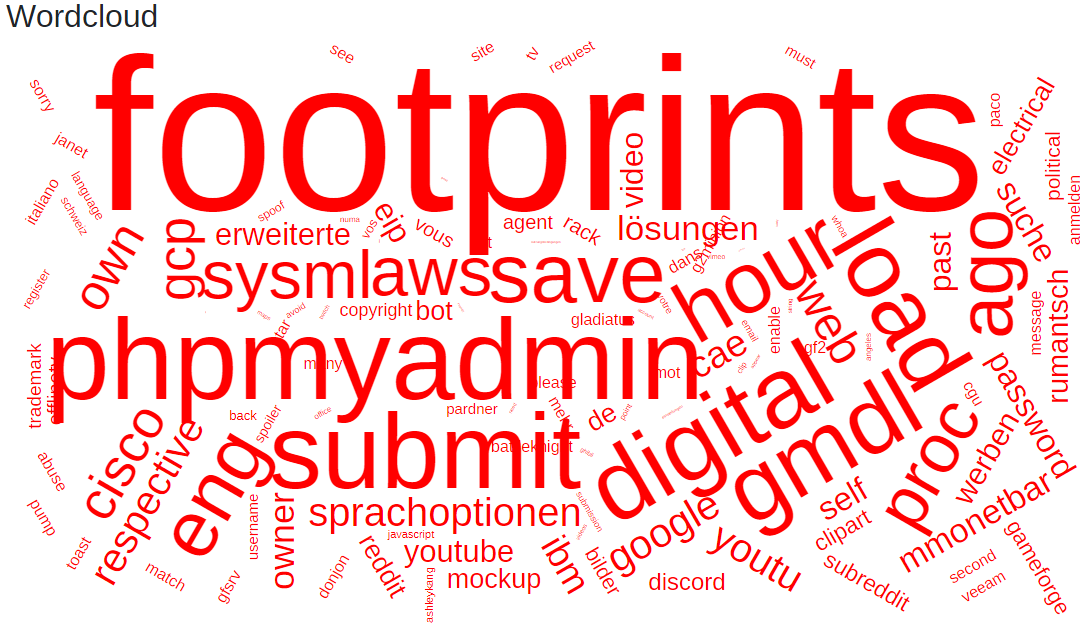
\includegraphics[width=1\textwidth]{images/results/critique-wordcloud}
			\caption{Vue de l'interface Wordcloud}
			\label{critique-wordcloud}
		\end{figure}

		Tout d'abord visuellement, cette vue remplit son objectif qui est de donner très rapidement une information sur les mots les plus représentatifs de l'utilisateur. En effet, les mots qui sont jugés les plus représentatifs sont affichés en plus grand, et ce sont également ceux vers lesquels l'oeil se pose en premier.

		Ensuite, les données représentées semblent correspondre avec la réalité de mon profil. Les mots que j'ai le plus consultés pendant la période durant laquelle j'ai conservé l'extension installée sont effectivement ceux qui sont le plus mis en valeur ici.

		En conclusion, cette vue assez simple me semble convenir dans à peu près tous les aspects car elle remplit tout à fait son rôle. La seule amélioration possible reste le choix d'une librairie graphique différente, pouvant éventuellement éviter le chevauchement de certains mots, cas qui apparaît ici plusieurs fois de manière non dérangeante, mais tout de même remarquable.

\FloatBarrier

		\subsubsection{Topics List}

		La figure~\ref{critique-topics} montre la vue de l'interface Topics List.

		\begin{figure}[!h]
			\centering
			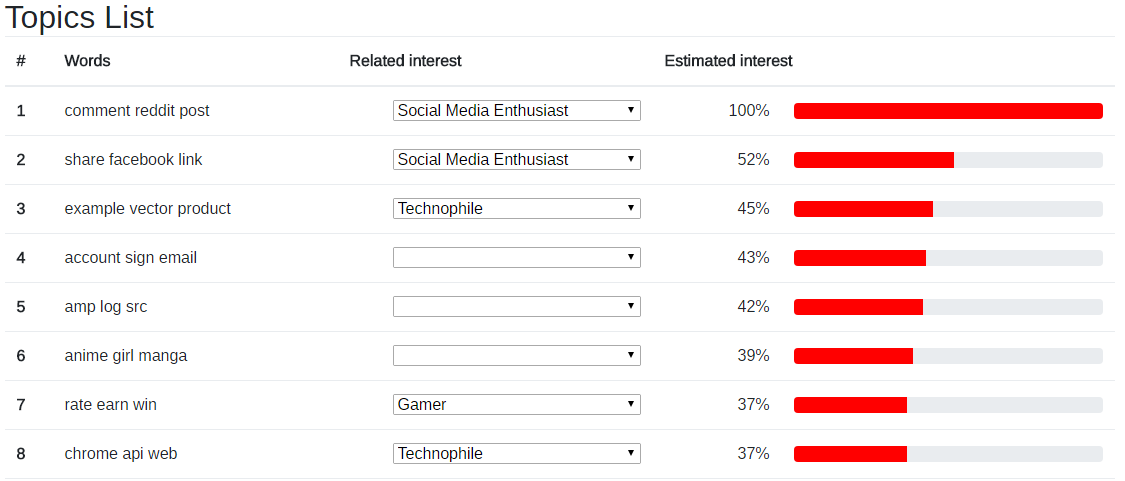
\includegraphics[width=1\textwidth]{images/results/critique-topics}
			\caption{Vue de l'interface Topics List}
			\label{critique-topics}
		\end{figure}

		On remarque ici que j'ai associé 5 des 8 meilleurs topics à certains de mes centres d'intérêt. Sur les 20 topics affichés sur la page, j'ai un total de 11 assignations. Ceci représente donc un taux de topics "corrects" légèrement supérieur à la moitié. Pour les 3 topics que j'ai laissé sans liens font ici :
		\begin{itemize}
			\item Représente un thème que je n'estime pas être important (account sign email)
			\item Fait peu de sens en soi (amp log src)
			\item Ne représente pas un thème auquel je m'identifie (anime girl manga)
		\end{itemize}

		En ce qui concerne le score d'intérêt estimé, seul le premier topic me parle vraiment, en le sens que je suis tout à fait d'accord et conscient que j'ai plus d'intérêt pour un topic défini par "comment reddit post" que les autres, probablement dû au fait de ma grande fréquentation du site reddit par rapport aux autres.

		J'arrive donc à expliquer l'énorme différence d'intérêt entre ce premier topic et les autres, et je le trouve correct. En revanche, je trouve que les différences minimes de pourcentage entre les autres topics fait peu de sens ; Je n'arriverais pas moi-même à les classer par ordre d'importance. Leur donner une valeur aussi précise me semble donc inutile, selon moi.

		Je trouve donc que les données représentées ici sont partiellement adéquates. Certaines d'entre elles sont pertinentes comme les mots des topics trouvés et une estimation de l'intérêt, même si les topics en eux-mêmes ne sont pas toujours corrects. En ce qui concerne la forme dont ces données sont présentées, je pense qu'une échelle avec une granularité diminuée serait moins confuse, par exemple un score de 1 à 5 pour chaque topic.

		Au final, je pense qu'il serait possible d'améliorer cette vue par deux ces moyens :
		\begin{itemize}
			\item Meilleure détection des topics d'intérêt
			\item Visualisation simplifiée du degré d'intérêt
		\end{itemize}

\FloatBarrier

		\subsubsection{Most watched and visited}

		La figure~\ref{critique-visited} montre la vue de l'interface Most Viewed, et la figure ~\ref{critique-watched} montre celle de l'interface Most Watched.

		\begin{figure}[!h]
			\centering
			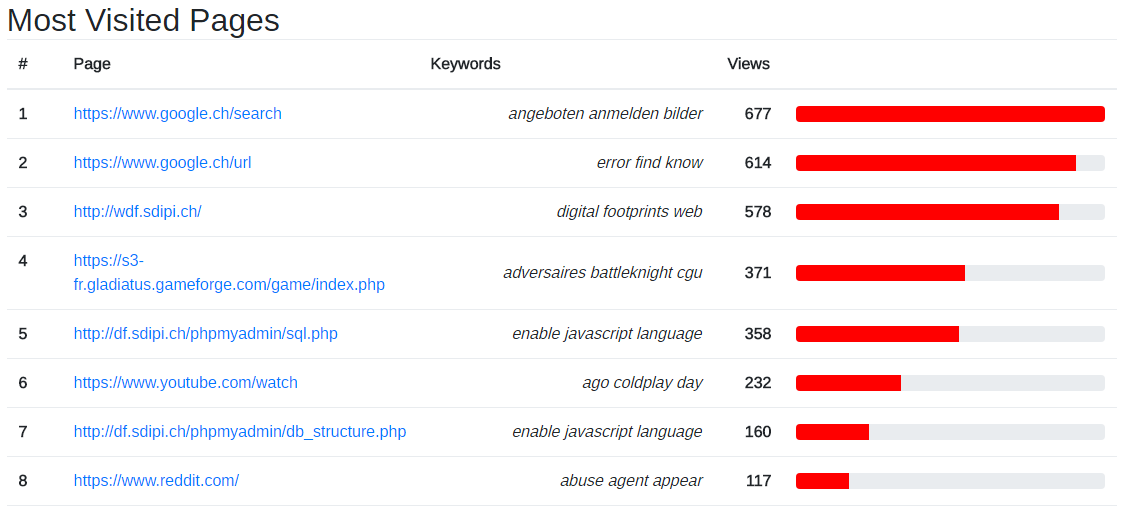
\includegraphics[width=1\textwidth]{images/results/critique-mostvisited}
			\caption{Vue de l'interface Most Visited}
			\label{critique-visited}
		\end{figure}

		\begin{figure}[!h]
			\centering
			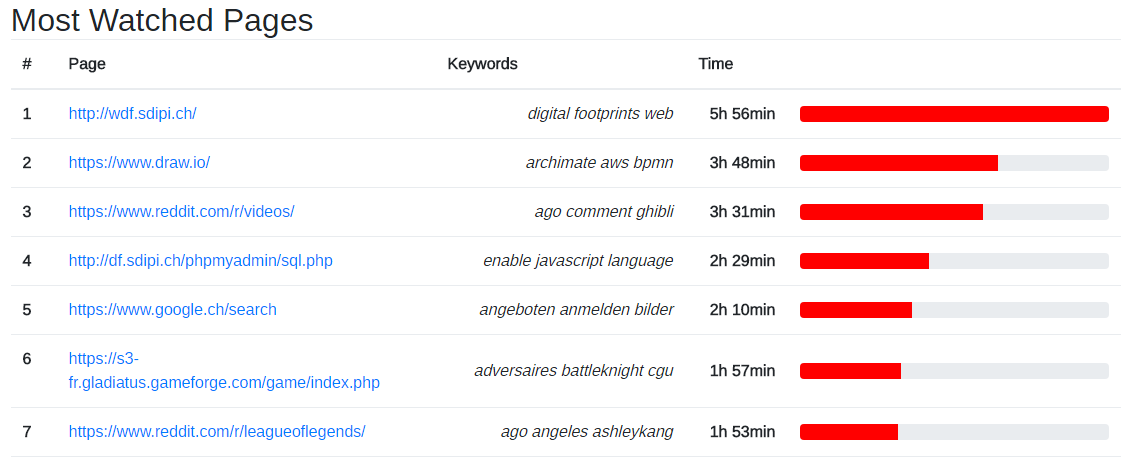
\includegraphics[width=1\textwidth]{images/results/critique-mostwatched}
			\caption{Vue de l'interface Most Watched}
			\label{critique-watched}
		\end{figure}

		À l'inverse des autres, ces deux vues-ci présentent des données qui n'ont pas été interprétées, ou en tout cas très peu. Le nombre de visites des pages web ne m'étonnent pas ni leur le temps passé sur celles-ci, je peux donc dire que je pense que ces données sur moi sont correctes.

		En ce qui concerne les "Keywords" trouvés, je trouve que plus de la moitié d'entre eux sont confus. Je trouve ceci dommage car je pense qu'il existe des meilleurs mots pour décrire les sites qui arrivent en tête des deux classements. Cependant, comme nous avons déjà expliqué dans un chapitre précédent les problèmes qui peuvent survenir pour détecter les mots idéaux sur certaines pages web, je remarque ici que les pages web que j'ai le plus visité sont des cas typiques de pages où il est difficile de déduire des mots clés idéaux.

		En effet, il s'agit principalement de pages web qui demandent une connection (comme wdf.sdipi.ch et draw.io), de pages web qui ne présentent pas ou peu de contenu texte (comme google.ch/search ou youtube.com), ou encore de pages web qui nécessiteraient l'URL non tronquée pour être correctement affichées (comme google.ch/url).

		Malheureusement, la plupart de ces cas ne semble pas montrer une résolution simple sans une acquisition de données supplémentaires. Il faudrait en effet que l'extension soit capable de voir le contenu effectivement affiché au client, et pas le contenu affiché de manière publique. Cette solution demanderait donc plus de données de la part de l'utilisateur, ce que nous avons volontairement évité.

		Au final, cette vue montre des informations quantitatives correctes comme le temps ou le nombre de visites, mais l'évaluation des mots des pages est peu précis. Le potentiel d'amélioration de cette vue se trouve probablement dans l'acquisition de données utilisateur supplémentaires.

\FloatBarrier

		\subsubsection{History}

		La figure~\ref{critique-history-topics} montre la vue de l'interface Wordcloud, et la figure ~\ref{critique-history-words} montre celle de l'interface Most Watched.

		\begin{figure}[!h]
			\centering
			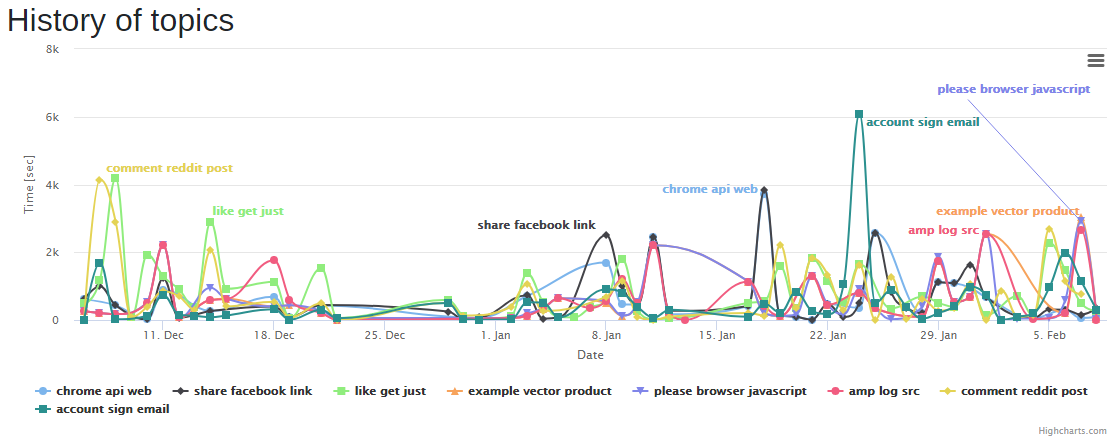
\includegraphics[width=1\textwidth]{images/results/critique-history-topics}
			\caption{Vue du premier graphique de l'interface History}
			\label{critique-history-topics}
		\end{figure}

		\begin{figure}[!h]
			\centering
			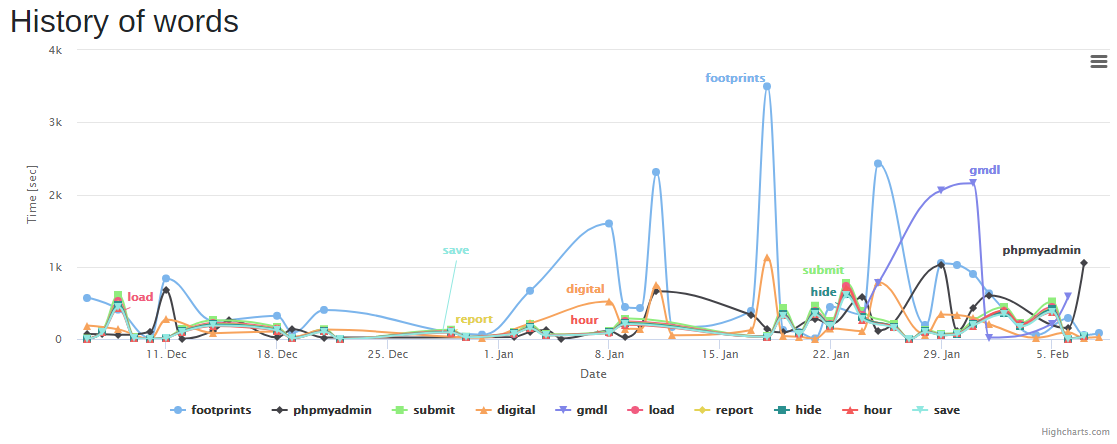
\includegraphics[width=1\textwidth]{images/results/critique-history-words}
			\caption{Vue du deuxième graphique de l'interface History}
			\label{critique-history-words}
		\end{figure}

		Tout d'abord visuellement, je pense que les vues montrent des tendances intéressantes, mais la quantité d'informations présentes entrave la lecture.

		En effet, on peut voir rapidement qu'il y a eu une période de pause entre le 23 décembre et le 3 janvier dans les deux graphiques. Cependant, il reste difficile d'isoler une tendance particulière pour un topic ou un mot particulier à première vue. La version web permet toutefois de cacher ou d'afficher des séries de données en cliquant dessus, ce qui permet d'alléger les graphiques.

		Je pense que l'information représentée est intéressante, mais qu'un travail supplémentaire sur la forme de la représentaiton pourrait valoir la peine. Par exemple, la possibilité de diminuer la granularité des points dans le temps, et de par exemple regrouper le temps passé à regarder certains mots ou topics peut être intéressant afin de voir plus clairement une tendance dans les deux visualisations.

\FloatBarrier

		\subsubsection{Trackers}

		La figure~\ref{critique-trackers} montre la vue de la page "Most recieving" de l'interface Trackers.

		\begin{figure}[!h]
			\centering
			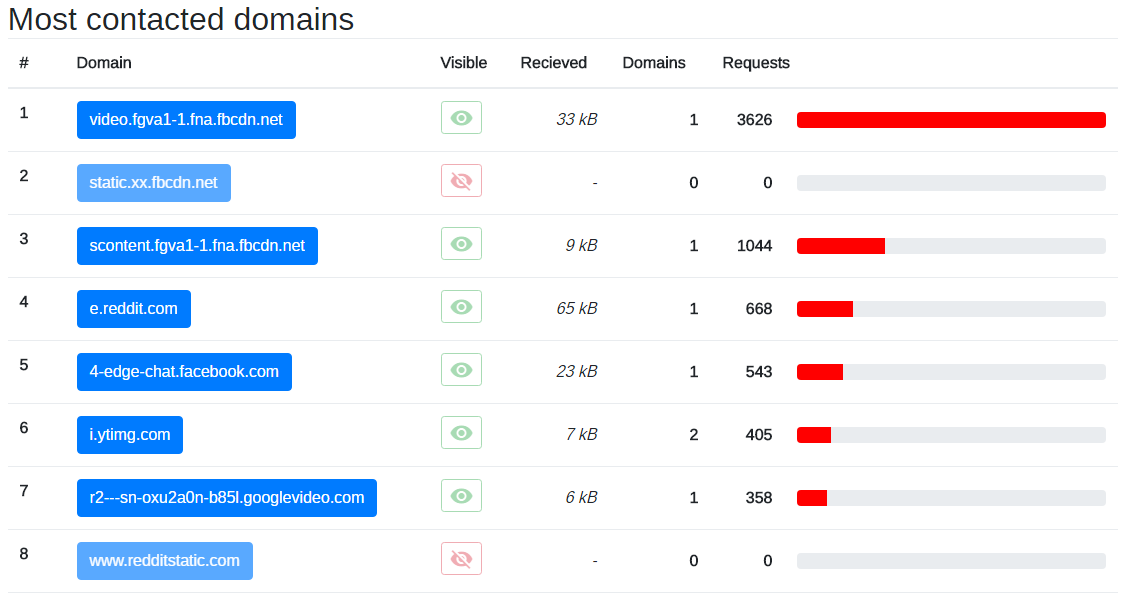
\includegraphics[width=1\textwidth]{images/results/critique-trackers}
			\caption{Vue de l'interface Wordcloud}
			\label{critique-trackers}
		\end{figure}

		La vue Trackers est celle qui présente le plus d'interactivité, et je me suis en effet pris au jeu d'essayer d'explorer les données en cachant certains domaines envoyant des données, puis certains autres domaines recevant les données, tout en vérifiant de temps en temps les détails de certains domaines.

		Il est difficile de juger des données présentes ici, car nous n'avons pas d'élément de comparaison. Le but de la vue Trackers est plutôt de faire découvrir  à l'utilisateur des informations qu'il ignorait lui-même sur sa navigation. Il est donc nécessaire ici de faire confiance à l'extension sur le traitement correct des informations.

		Visuellement et interactivement, je trouve que cette vue est particulièrement réussie. J'ai pu naviguer à travers elle et découvrir des nouvelles informations sur ma navigation de manière assez aisée et tout semble clair.

		Les possibilités d'amélioration de cette vue sont principalement l'ajout d'une ou deux fonctionnalités supplémentaires d'ergonomie : Par exemple la possibilité de trier les domaines par colonne faciliterait un peu la synthèse des données présentées.

		\subsubsection{Conclusion}

			D'une manière générale, j'ai trouvé que les données représentées correspondent assez bien à mon profil, ou du moins à ce que j'imagine que ma navigation dévoile de mon profil. Des modifications et des améliorations dans la manière dont sont traitées les données peuvent sans aucun doute augmenter la fidélité apparente avec laquelle le profil est généré, car certaines informations déduites sont tout de même très imprécises, comme les keywords de mes pages les plus vues.

			Cependant malgré les imperfections, je peux dire avec confiance que je me reconnais dans la plupart des informations qui me sont présentées vie l'interface.

\section{Statistiques}

	Un total de 10 utilisateurs volontaires ont installé l'extension, dont 8 d'entre eux ont été identifiés comme ayant une activité de navigation sur Chrome assez grande pour contribuer à l'étude. Bien que la taille de l'échantillon soit peu impressionnante, le fait que ceux-ci aient utilisé l'extension pendant environ 1 mois nous permet tout de même de montrer des statistiques.

	En effet, la taille de la base de données finale est d'environ 4.5 Gio. La moitié de ces données sont le stockage du contenu des pages, l'autre moitié est remplie par des données sur les utilisateurs. Voici ce que nous pouvons dire sur ces données après les avoir analysées.

	Tout d'abord, quelques statistiques générales. La figure~\ref{r-visionnage} montre le temps passé total à visualiser des pages par domaine. On remarque déjà à cette étape certaines tendances de notre audience.

	\begin{figure}[!h]
		\centering
		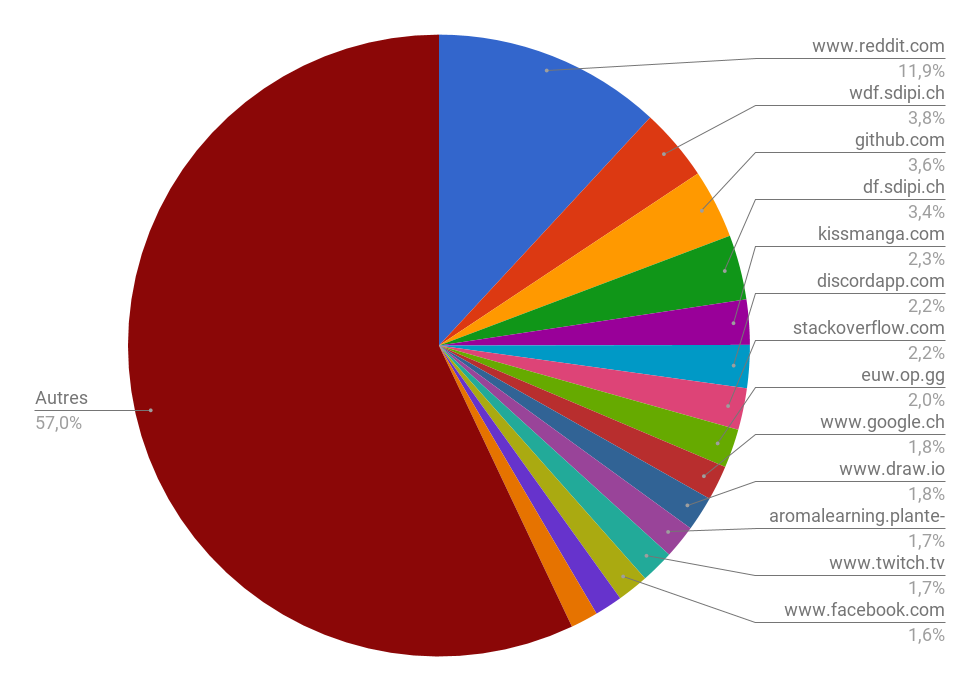
\includegraphics[height=0.75\textwidth]{images/results/temps_total_visionnage}
		\caption{Temps total de visionnage par domaine}
		\label{r-visionnage}
	\end{figure}

	\subsection{Profiling}

		Pour chacun des utilisateurs qui a renseigné ses centres d'intérêt dans son profil, nous nous sommes intéressé à la correspondance entre les profils que les utilisateurs ont renseigné, et les topics que nos algorithmes ont estimé être intéressants pour eux.

		\subsubsection{Résultats généraux}

		\subsubsection{Critique}

		\subsubsection{Conclusion}

	\subsection{Trackers}

		Un total de 3'227'000 requêtes ont été enregistrées dans la table \texttt{pagerequests}, représentant environ 1 Gio de données. 

		\subsubsection{Requêtes envoyées}

			<Nombre de requêtes envoyées par visite, par URL>

			<Nombre de requêtes envoyées par minute, par URL>

		\subsubsection{Requêtes reçues}

			<Nombre de requêtes reçues par visite, par URL>

			<Nombre de requêtes reçues par minute, par URL>

		\subsubsection{Autres statistiques}

			<Trackers contacté par le + de domaines différents>

			<Domaines envoyant la plus grosse quantité de donnéespar requête> 
